\label{research}
So far, we discussed an extension of the pilot abstraction to support data analytics and task based data intensive applications on HPC resources, a comparison between different task-based data oriented frameworks, and a design comparison for executing scientific workflows.
In this section, we motivate and propose a Campaign Manager (CM) to execute scientific campaigns via creating and enacting a campaign execution plan on heterogeneous and dynamic HPC resources. \mtnote{Do we need to explain how these three topics fit together?}\gpnote{I am not sure}

\subsection{Proposed Topic}
Scientific campaigns execute workflows on heterogeneous resources either with a given objective~\cite{casajus2010dirac} and/or for large periods of time~\cite{maeno2008panda}.\mtnote{I think the two are not mutually exclusive: executions of campaigns can have both a given objective and run for a large period of time.}
This objective can be translated to a computational objective function that would either minimize or maximize a metric.
Calculating the makespan of the campaign means finding the execution plan that satisfies the computational objective function.


\mtnote{Following the work we did on the separated scratch document, here a brief summary of the 'story' we agreed upon: 
\begin{enumerate}
    \item  General description of the problem space in terms of homo/heterogeneity of campaigns' workflows/resources with the help of the diagram in Figure 1, iterated to show the relevance of space heterogeneity; 
    \item initial formal definition of TTX\_w, including revised list of explicit assumptions, argument about abstraction from resource implementation, list of symbols, and first three equations (r=1, w=\{space/time homo*, space/time hetero*\}; r=n,  w=\{space/time homo*\}; r=n,  w=\{time hetero*\}); 
    \item propose to expand this initial model in the next year by: 
    \begin{enumerate}
        \item relax assumption about homogeneous resources; 
        \item add type heterogeneity of both r and w; 
        \item define m algorithmically; 
        \item if there is time, propose a quantitative definition of m.
    \end{enumerate}
\end{enumerate}}
\gpnote{moved it here}

The way workflows of a given campaign are mapped to resources can affect the makespan of the campaign. 
Figure~\ref{fig:example_makespan} shows an example of a campaign with heterogeneous workflows, and the makespan two different mappings produce.
The makespan of the campaign on the left subfigure is $20$, while on the right it is $16$.
In addition, the size of the workflows, i.e., the number of resources they require, becomes relevant and resources may be underutilized, as shown in Figure~\ref{fig:example_makespan}.

\begin{figure*}[ht!]
    \centering
    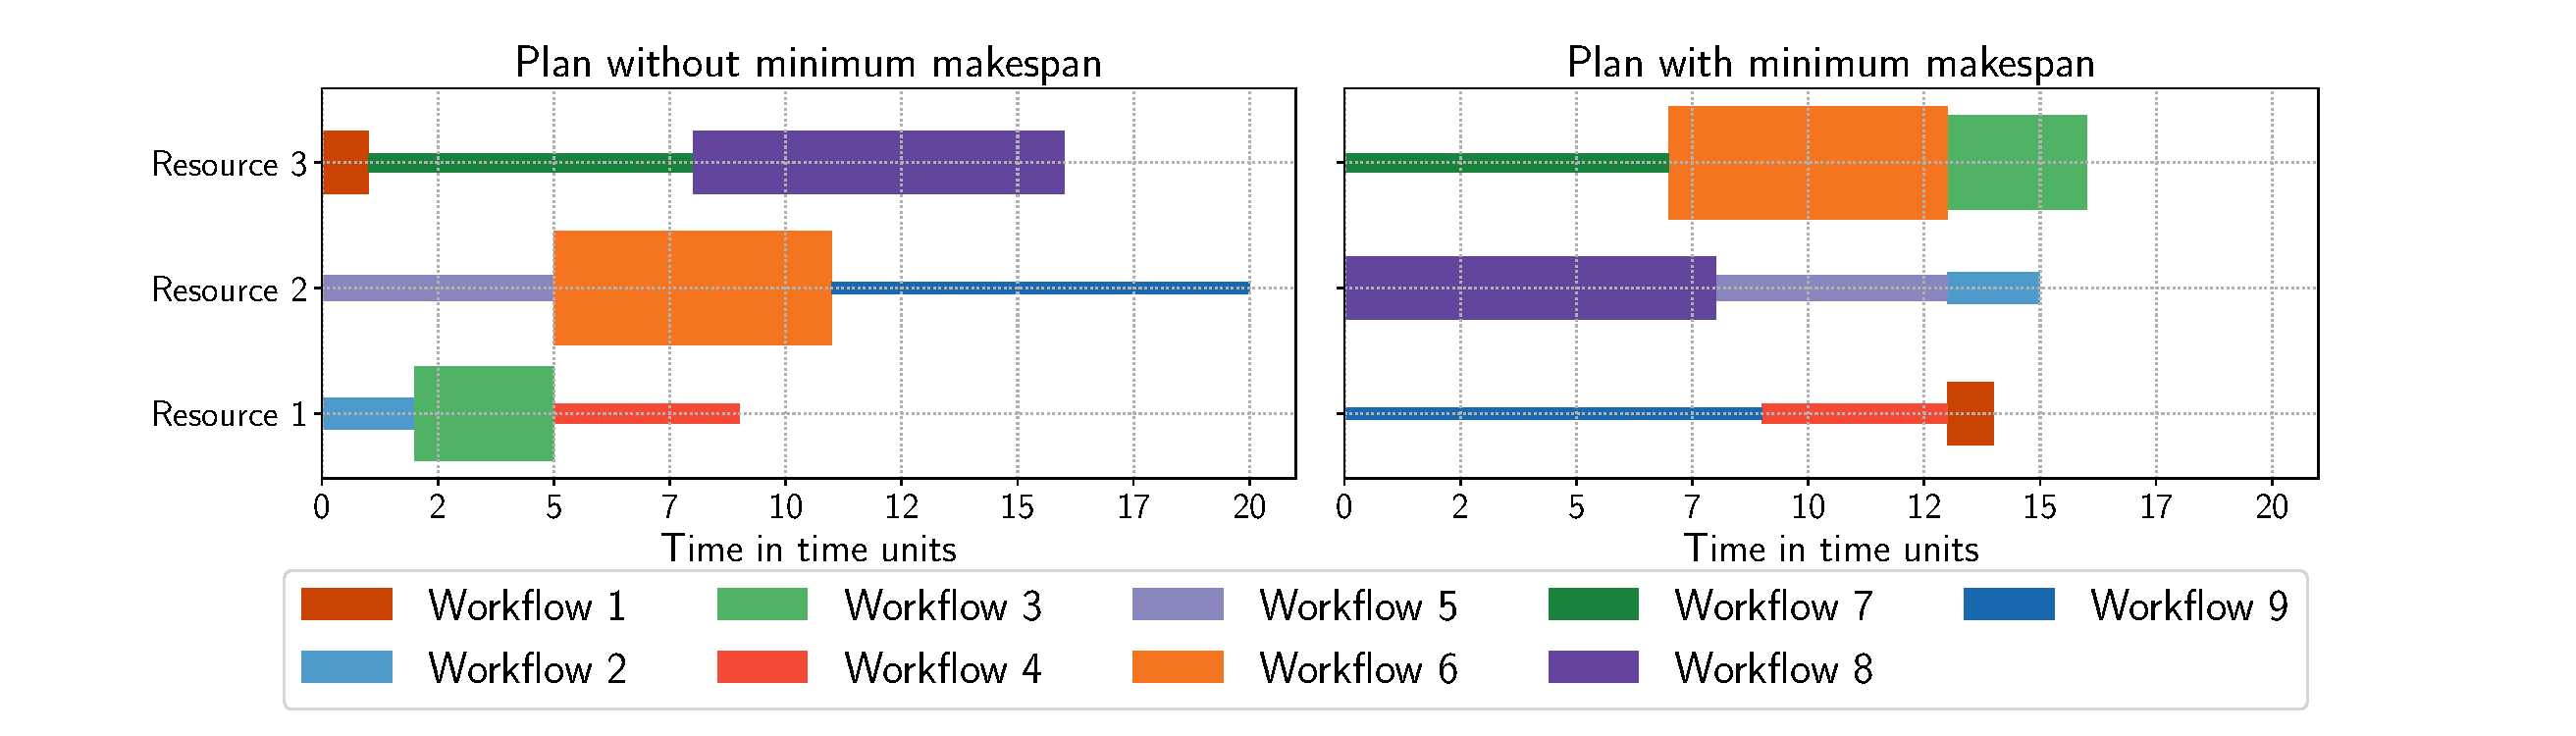
\includegraphics[width=.95\textwidth]{figures/random_vs_specific.pdf}
    \caption{Random plan versus minimum makespan plan}\label{fig:example_makespan}
\end{figure*}

We are making a set of assumptions which we do not relax during our initial analysis.
These are:
\begin{inparaenum}[(1)]
    \item a workflow is an atomic unit and cannot be decomposed;
    \item workflow resource request is sufficient to execute the workflow and the requested resources are utilized;
    \item a resource is an aggregate of computing capabilities;
    \item every workflow of a given campaign can be executed;
    \item a random resource selection is based on a uniform distribution;
    \item only one workflow can be executed on a resource at any point in time; and
    \item a workflows can be homogeneous or heterogeneous in space---maximum number of resources they need, and time---the amount of time they are executing.
\end{inparaenum}

We denote a computational campaign as $w = [w_{i}: 1 \leq i \leq W]$, where $w_{i}$ is a workflow and $W$ is the total number of workflows, $r = [ r_{j}: 1 \leq j \leq R]$ is a set of available resources, where $r_{j}$ is a resource and $R$ is the total number of available resources, and $ m(w,r) = [(w_i, r_j): 1 \leq i \leq W, r_j \in r] $ is a mapping function of workflows onto resources.
In addition, we denote as $TTX_{w_{i}}$ the execution time of a workflow, $TTX_{w}$ as the makespan of campaign $w$, and $TTX_{w}^{m}$ as the makespan of campaign $w$ for a given mapping function $ m $.
Assumption~\#3 allows to abstract the resource implementation, as workflows can be executed on different resources such as HPCs, Clouds, pilots and more. 
Lastly, we will assume homogeneous resources as it simplifies the formalization of the problem.

Assuming a single resource, i.e., $R = 1$, the workflows of the campaign will be executed sequentially, whether the workflows are homogeneous or heterogeneous.
As a result the makespan of the campaign is
\begin{equation}
   TTX_{w} = \sum_{i=1}^{W}TTX_{w_{i}} 
\end{equation}

When assuming multiple homogeneous resources, i.e., $1 < R < W$, the workflows can be executed concurrently.
Furthermore, this is semantically equivalent to executing on a single resource large enough to allow concurrent workflow execution, where each workflow executes on resource partition. 
Because of assumptions~\#4 and~\#6, executing homogeneous workflows or heterogeneous in space workflows is the same.
A random mapping of workflows onto resource will have a makespan
\begin{equation}
   TTX_{w}^{random} \geq \frac{1}{R}\sum_{i=1}^{W} TTX_{w_{i}} 
\end{equation}
When executing workflows heterogeneous in time, whether they are heterogeneous in space or not as well, on multple homogeneous resources, the makespan of the campaign for a given mapping function $ m $ is

\begin{equation}
TTX_{w}^{m} = \max_{r_{j}\in r}\Big\{\sum_{r_{i}\in m(w,r_{j})}TTX_{w_{i}}\Big\}
\label{eq:makespan}
\end{equation}

During the next year, we propose to expand the model, as it is represented in equation~\ref{eq:makespan}, by relaxing some of the initial assumptions.
First, we will relax the assumption that resources are homogeneous in terms of (1) maximum number of resources they have available; (2) type of resources, e.g., CPUs or GPGPUs; and (3) the time they are available.
Second, we will add resource type heterogeneity of workflows.
As a result, workflows will not be able to be executed on all available resources affecting the way the makespan is being calculated.
Furthermore, we propose to explore algorithmic instances of the mapping function $ m $, and if there is time, we will propose a quantitative definition of $ m $.

\mtnote{I think that we will need either equations or diagrammatic representation of the placement + makespan, ideally both. Even knowing quite well what you are trying to write, it is very difficult to follow your argumentation. There are elements of the argumentation (assuming I understand it well enough) that I might disagree with but I am going to keep those thoughts for after the proposal :)}
\gpnote{separate document moved here.}

% ----------------------------------------------------------------------------
% campaign makespan modeling
We propose to utilize and extend the Heterogeneous Earliest Finish Time (HEFT)~\cite{topcuoglu2002performance} algorithm  as an initial candidate of the mapping function $ m $\mtnote{for doing what?}\gpnote{any better?}.
HEFT is an offline scheduling algorithm which calculates the makespan of a workflow on heterogeneous resources, in terms of performance.
HEFT has been implemented as part of the planning capabilities in Pegasus~\cite{deelman2015pegasus} and ASKALON~\cite{fahringer2005askalon} amongst other algorithms.
HEFT provided better performance in terms of makespan minimization when compared to a random or round robin plan~\cite{deelman2015pegasus}.
This makes HEFT a good candidate for minimizing the makespan of a campaign.


HEFT makes two important assumptions when used to work upon workflows.
First, any task in a workflow can be executed in all available resources, and second all resources are always available.
HEFT is mainly used to derive and execution plan for workflows, i.e. the execution order and resource placement of the tasks that comprise the workflow.
Because we are interested in campaigns, our HEFT extension will provide an execution plan based on workflows as the unit it will operate.
HEFT uses a matrix to represent execution time of tasks on resources, assigning tasks to the resource that minimizes the finish time of the task, and has complexity proportional to the number of dependencies between tasks and the number of resources offered.\mtnote{Why suddenly are we writing about tasks? What is the relationship between HEFT, tasks, workflows and campaigns?}\gpnote{HEFT was created to work on workflows. I added the next paragraph to show how HEFT for campaigns might be different.}
Furthermore, there has been some initial research to extend HEFT to resources that provide CPU and GPUs~\cite{shetti2013optimization}, as well as a HEFT extension on dynamic resources~\cite{dong2007pfas}.

We identify four points of possible extensions, so that HEFT is utilized for campaigns.
These are:
\begin{inparaenum}[(i)]
    \item selecting resource that can execute a given workflow,
    \item taking into account dynamic resources, as they may become unavailable during execution,
    \item multiple workflows may be executed in a single resource concurrently, and
    \item including user specified priorities for workflows.
\end{inparaenum}
Because workflows are heterogeneous, we assume that there is at least one resource can satisfy the computational requirements of any workflow in the campaign, but not necessarily all resources.
Resources may become unavailable because the user has no allocation left, a scheduled maintenance is taking place, or due to some unscheduled downtime.
During the execution of a campaign, some workflows may have a higher priority compared to other due to user preference, or as response to an unforeseen event.
As a result, HEFT's data structure and HEFT needs to be extended to identify whether a workflow can be executed in a given resource or not, whether a resource is available or not, and user provided initial priorities.
Finally, a resource may have enough capacity so that multiple workflows can be executed concurrently.
We will investigate how HEFT can be extended to support variable resource capacity.\gpnote{It may need further extension.}

There are several alternative methods and algorithms to calculate and optimize the makespan of a workflow~\cite{lu2019review}, including queuing networks~\cite{yao2019throughput,bao2019performance}, domain specific languages~\cite{carothers2017durango,maheshwari2016workflow}, and machine learning~\cite{witt2019predictive,pumma2017runtime}.
Queuing networks will be of limited use because they require from the user to provide a queuing network equivalent to the campaign.
In the case the campaign contains only independent workflows, a single queuing system with multiple servers would be sufficient, but a campaign with complex dependencies between workflows may require expertise outside of the user domain to define the equivalent queuing network.
HEFT sorts workflows based on the number of dependencies they have in the campaign.
Furthermore, using queuing systems to derive the makespan of a campaign requires to search for possible mappings and keep the one that optimizes the makespan.
HEFT provides as an output, the plan that minimizes the makespan.
\mtnote{These two sentences are unclear, please revise.}\gpnote{any better?}
Domain specific languages approaches either require description of the resource usage of workflows~\cite{carothers2017durango}, or execute part of the campaign to obtain execution skeleton of the campaign~\cite{maheshwari2016workflow}.
When executing a campaign, workflows may require days to execute to obtain execution time information, and users rarely know the resource usage of their workflows to provide enough useful information.
In addition, the workflows of a campaign may be different and executing some of them may not provide any information about the execution of others.
HEFT also requires an initial estimation of the execution time of the workflows. We plan to utilize initial estimations provided by the users and update the values as workflows are being executed.
\mtnote{This is unconvincing: we choose to use the PST model and then we say that it requires too much effort? Remember: the argumentation here has to be `scientific', not just based on 'I want to use EnTK so this would require too much time'.}\gpnote{I removed the EnTK argument.}
Similarly, machine learning approaches would be of limited use since there is no guarantee that the workflows of a campaign is are going to be similar.
As a result, to gather enough information to build a makespan calculation model may require the execution of the campaign.\mtnote{Why would this be a problem?}\gpnote{changed it}.
We want to provide an approach that only requires the user to provide as few information as possible, such as the workflows and an educated guess of their execution time\gpnote{any better?}.

% ----------------------------------------------------------------------------
% Campaign Manager definition, requirements, features and capabilities
We propose to design a campaign manager (CM) which, given a campaign, an objective, and a set of constraints, can derive an execution plan by utilizing the proposed makespan HEFT algorithm, and execute a campaign.
If necessary the CM will change the execution plan by updating workflow to resource mapping, and resource availability.
Execution planning for workflows are provided by several workflow execution systems, such as Pegasus~\cite{deelman2015pegasus}, and ASKALON~\cite{fahringer2005askalon}.
Campaign management systems, such as PanDA~\cite{maeno2008panda}, do not provide a campaign planning feature.
QCFractal~\cite{qcfractal} offers some form of planning by allowing user to specify the priority of a workflow in a campaign, but it does not plan with taking into account the makespan of the campaign.\mtnote{only these two among all the existing systems? Please refine and expand, explaining that these are just examples. Also, expand appropriately introducing the notions of planning and plan and explaining why they relate to campaign management.}\gpnote{I introduced the plan a few paragraphs before. It may still need to be expanded.}

Figure~\ref{fig:refarch} shows a reference architecture where the CM has three components:
\begin{inparaenum}[(1)]
\item a Planner,
\item and Enactor, and
\item a Bookkeeper. 
\end{inparaenum}
Workflow execution will be done through an existing workflow management framework (WMF) on HPC resources.
Plan updates will be based on workflows execution metrics provided by the selected WMF such as tasks execution time, overheads calculation and time to completion.
These metrics will be aggregated across workflows resulting in campaign-wide execution metrics.

\begin{figure*}[t]
    \centering
    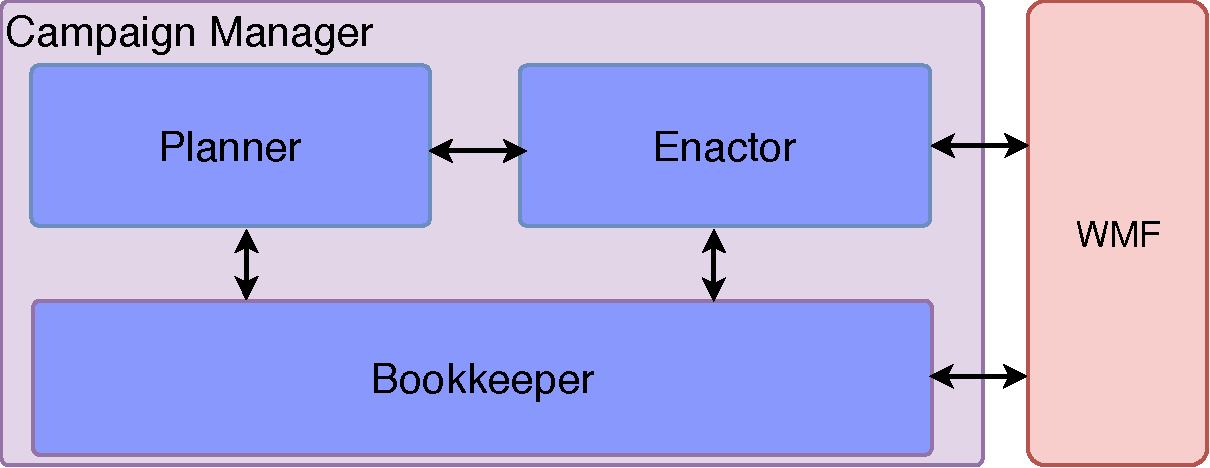
\includegraphics[width=.95\textwidth]{figures/CEM_design.pdf}
    \caption{Reference Architecture of a Campaign Manager. Basic 
    components of Campaign Manager (CM): 1) Planner, 2) Enactor and 3) Bookkeeper. 
    CM communicates decisions to RADICAL-EnTK. CM communicates with HPCs to 
    execute parts of the campaign.}\label{fig:refarch}
\end{figure*}

The Planner is responsible to derive an execution plan by calculating\mtnote{is it a calculator or an optimizer? Seem different capabilities to me and not necessarily part of the same component}\gpnote{any better?} the makespan of a campaign based on a set of resources, and an objective, via utilizing the extend HEFT algorithm. \mtnote{It seems to me that makespan calculation is only one of the elements needed to derive a plan. As such, I think you need at least two components in your architecture: makespan calculator and planner.}\gpnote{The planner uses the makespan calculation to derive a plan. I do not think they should be two different components.}
The planner pulls from the bookkeeper information about the state of resources as well as the state of the workflows of the campaign.
In addition based on information from the other components, the planner may update the plan accordingly. 

The Bookkeeper component is responsible to monitor the execution of the campaign.
This component knows the state of the campaign, the execution plan, the availability of the resources, and the campaign's objective.
The state of the campaign is based on information that the bookkeeper receives from the used WMF and the enactor component.
In addition, it knows the state of the resources the campaign is utilizing or will utilize.
Based on this set of information, it checks whether the campaign's objective can be achieved.
If any change in the campaign happens, such as workflows are added or removed, a resource is not available, or the objective is not going to be met, the bookkeeper informs the planner to update the plan.
An important feature of the bookkeeper is to identify the reason of a failing workflow.
When the failure is because the resource is not available, the specific workflow may need to be executed and the plan to be updated.

The Enactor is responsible to execute the plan decided by the planner by interfacing with the WMF.
Based on the plan, the enactor is responsible to execute workflows on the respective resources based on the plan.
To achieve that, the enactor informs the WMF to acquire resources, translates the workflow from the user's specification to the API provided by the WMF, and submits the workflow.
In the case where a group of workflows is to be executed as a single workflow, the enactor is responsible to group them as well.
Furthermore, it informs the bookkeeper which workflows were submitted for execution.



Scientific workflows are mainly executed by utilizing dedicated workflow management frameworks (WMF), such as RADICAL-Ensemble Toolkit~\cite{balasubramanian2018harnessing}, Pegasus~\cite{deelman2015pegasus} and others.
These frameworks offer runtime capabilities, such as task execution, data dependency resolution, and workflow definition and monitoring.
Given a set of resources and a walltime, WMF try to maximize resource utilization and minimize time to completion.
WMF assume that the user selects sufficient resources and walltime to execute the workflow.
Some workflow management frameworks, such as Dask~\cite{rocklin2015dask} and Airflow~\cite{airflow}, provide capabilities to elastically adapt resources, by scaling up or down, based on the current state of execution.
In addition, some  WMFs~\cite{deelman2015pegasus} may support the concurrent execution of multiple workflows as independent entities, but not a single unified entity to achieve a single objective.

RADICAL-Ensemble Toolkit~\cite{balasubramanian2018harnessing} (EnTK) is a workflow management framework.
We selected to utilize EnTK because it fits the requirements of the target use cases, and it utilizes a pilot framework as its runtime system.
EnTK defines workflows as a set of pipelines, each pipeline is a sequence of stages, and in turn each stage a set of tasks.
Concurrency during execution happens at the level of pipelines and tasks.
Furthermore, EnTK supports the execution of a sequence of workflows by either reusing already acquired resources or by requesting new ones\mtnote{grammar: from `may' onwards I do not understand the sentence anymore.}\gpnote{fixed it}.
EnTK workflow execution is stateful, provides execution timing traces for tasks and workflows, and supports workflow execution on multiple HPC resources.
Furthermore, EnTK utilizes a pilot runtime system, RADICAL-Pilot~\cite{merzky2019using}, to execute workflows on HPC resources.
Pilot systems submit job placeholders on resources, and are able to execute tasks on the acquired resources.
This capability allows to execute multiple workflows to resources that are acquired once, either sequentially or concurrently.
The proposed campaign manager will interface with EnTK through the enactor and bookkeeper components to execute and monitor workflows based on the derived execution plan.

\mtnote{General note: this needs to be expanded following the comments I left. At the moment, a lot of this still reads as a set of sometimes disconnected statements. We need to iterate so to produced a more detailed description of the research you propose to conduct in the next year, a description backed by existing literature and your own argumentation. From our discussions, I know you have the material needed to iterate this initial draft.}\gpnote{Let me know how much this comment still holds.}
